\chapter{Конструкторская часть}

В данном разделе представлены схемы алгоритмов умножения матриц и выполнена оценка их трудоёмкости.

\section{Представление алгоритмов}

Алгоритм принимает на вход две матрицы: $mtr1$ размера $N \times M$, $mtr2$ размера $M \times T$, где $M, N, T$ --- неотрицательные целые числа; на выходе --- результат умножения двух матриц, записанный в $res$ размера $M \times K$.

Оптимизированная версия алгоритма Винограда предусматривает следующие изменения:

\begin{itemize}
	\item[---] использование побитового сдвига целого числа вместо умножения на 2;
	\item[---] объеденение IV и III частей алгоритма, избавившись от совпадающей пары циклов;
\end{itemize}

На~рис.~\ref{fig:shemanum1}--\ref{fig:shemanum3} приведены схемы стандартного алгоритма умножения матриц, алгоритма Винограда и оптимизированного алгоритма Винограда.

\clearpage

\begin{figure}[h]
	\centering
	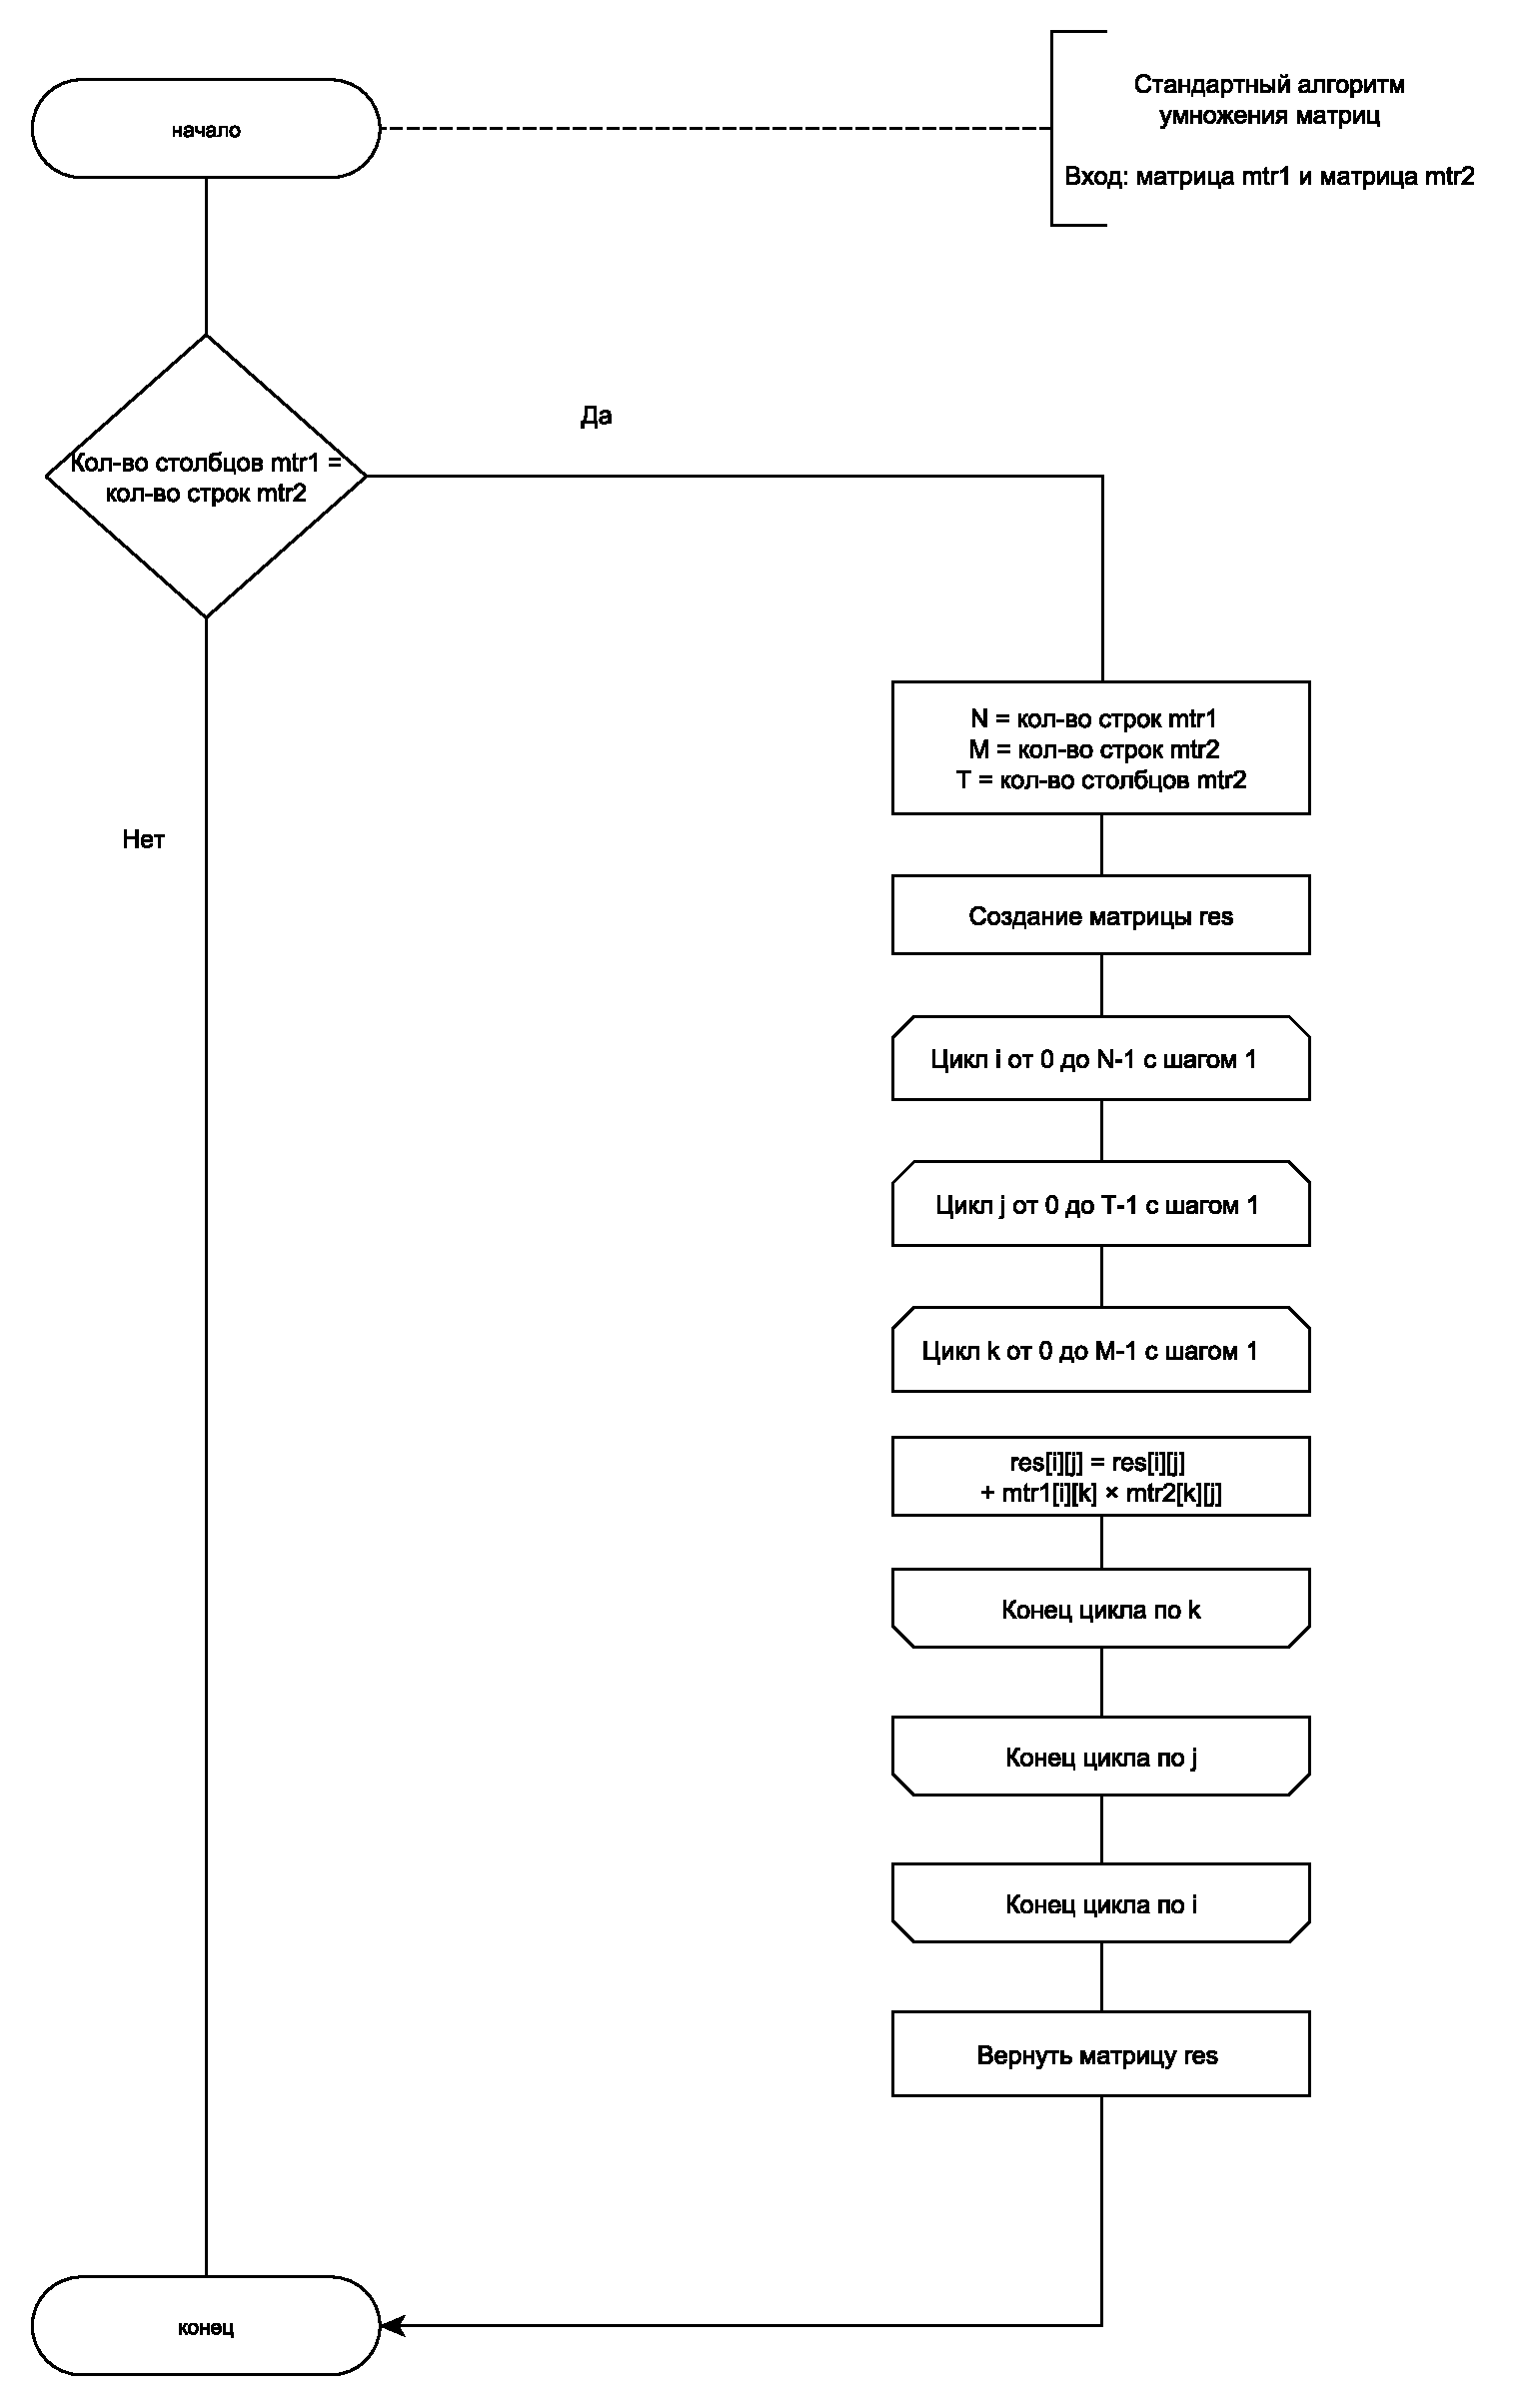
\includegraphics[width=0.8\linewidth]{images/shema_num1}
	\caption{Схема классического алгоритма умножения матриц}
	\label{fig:shemanum1}
\end{figure}

\clearpage

\begin{figure}[h]
	\centering
	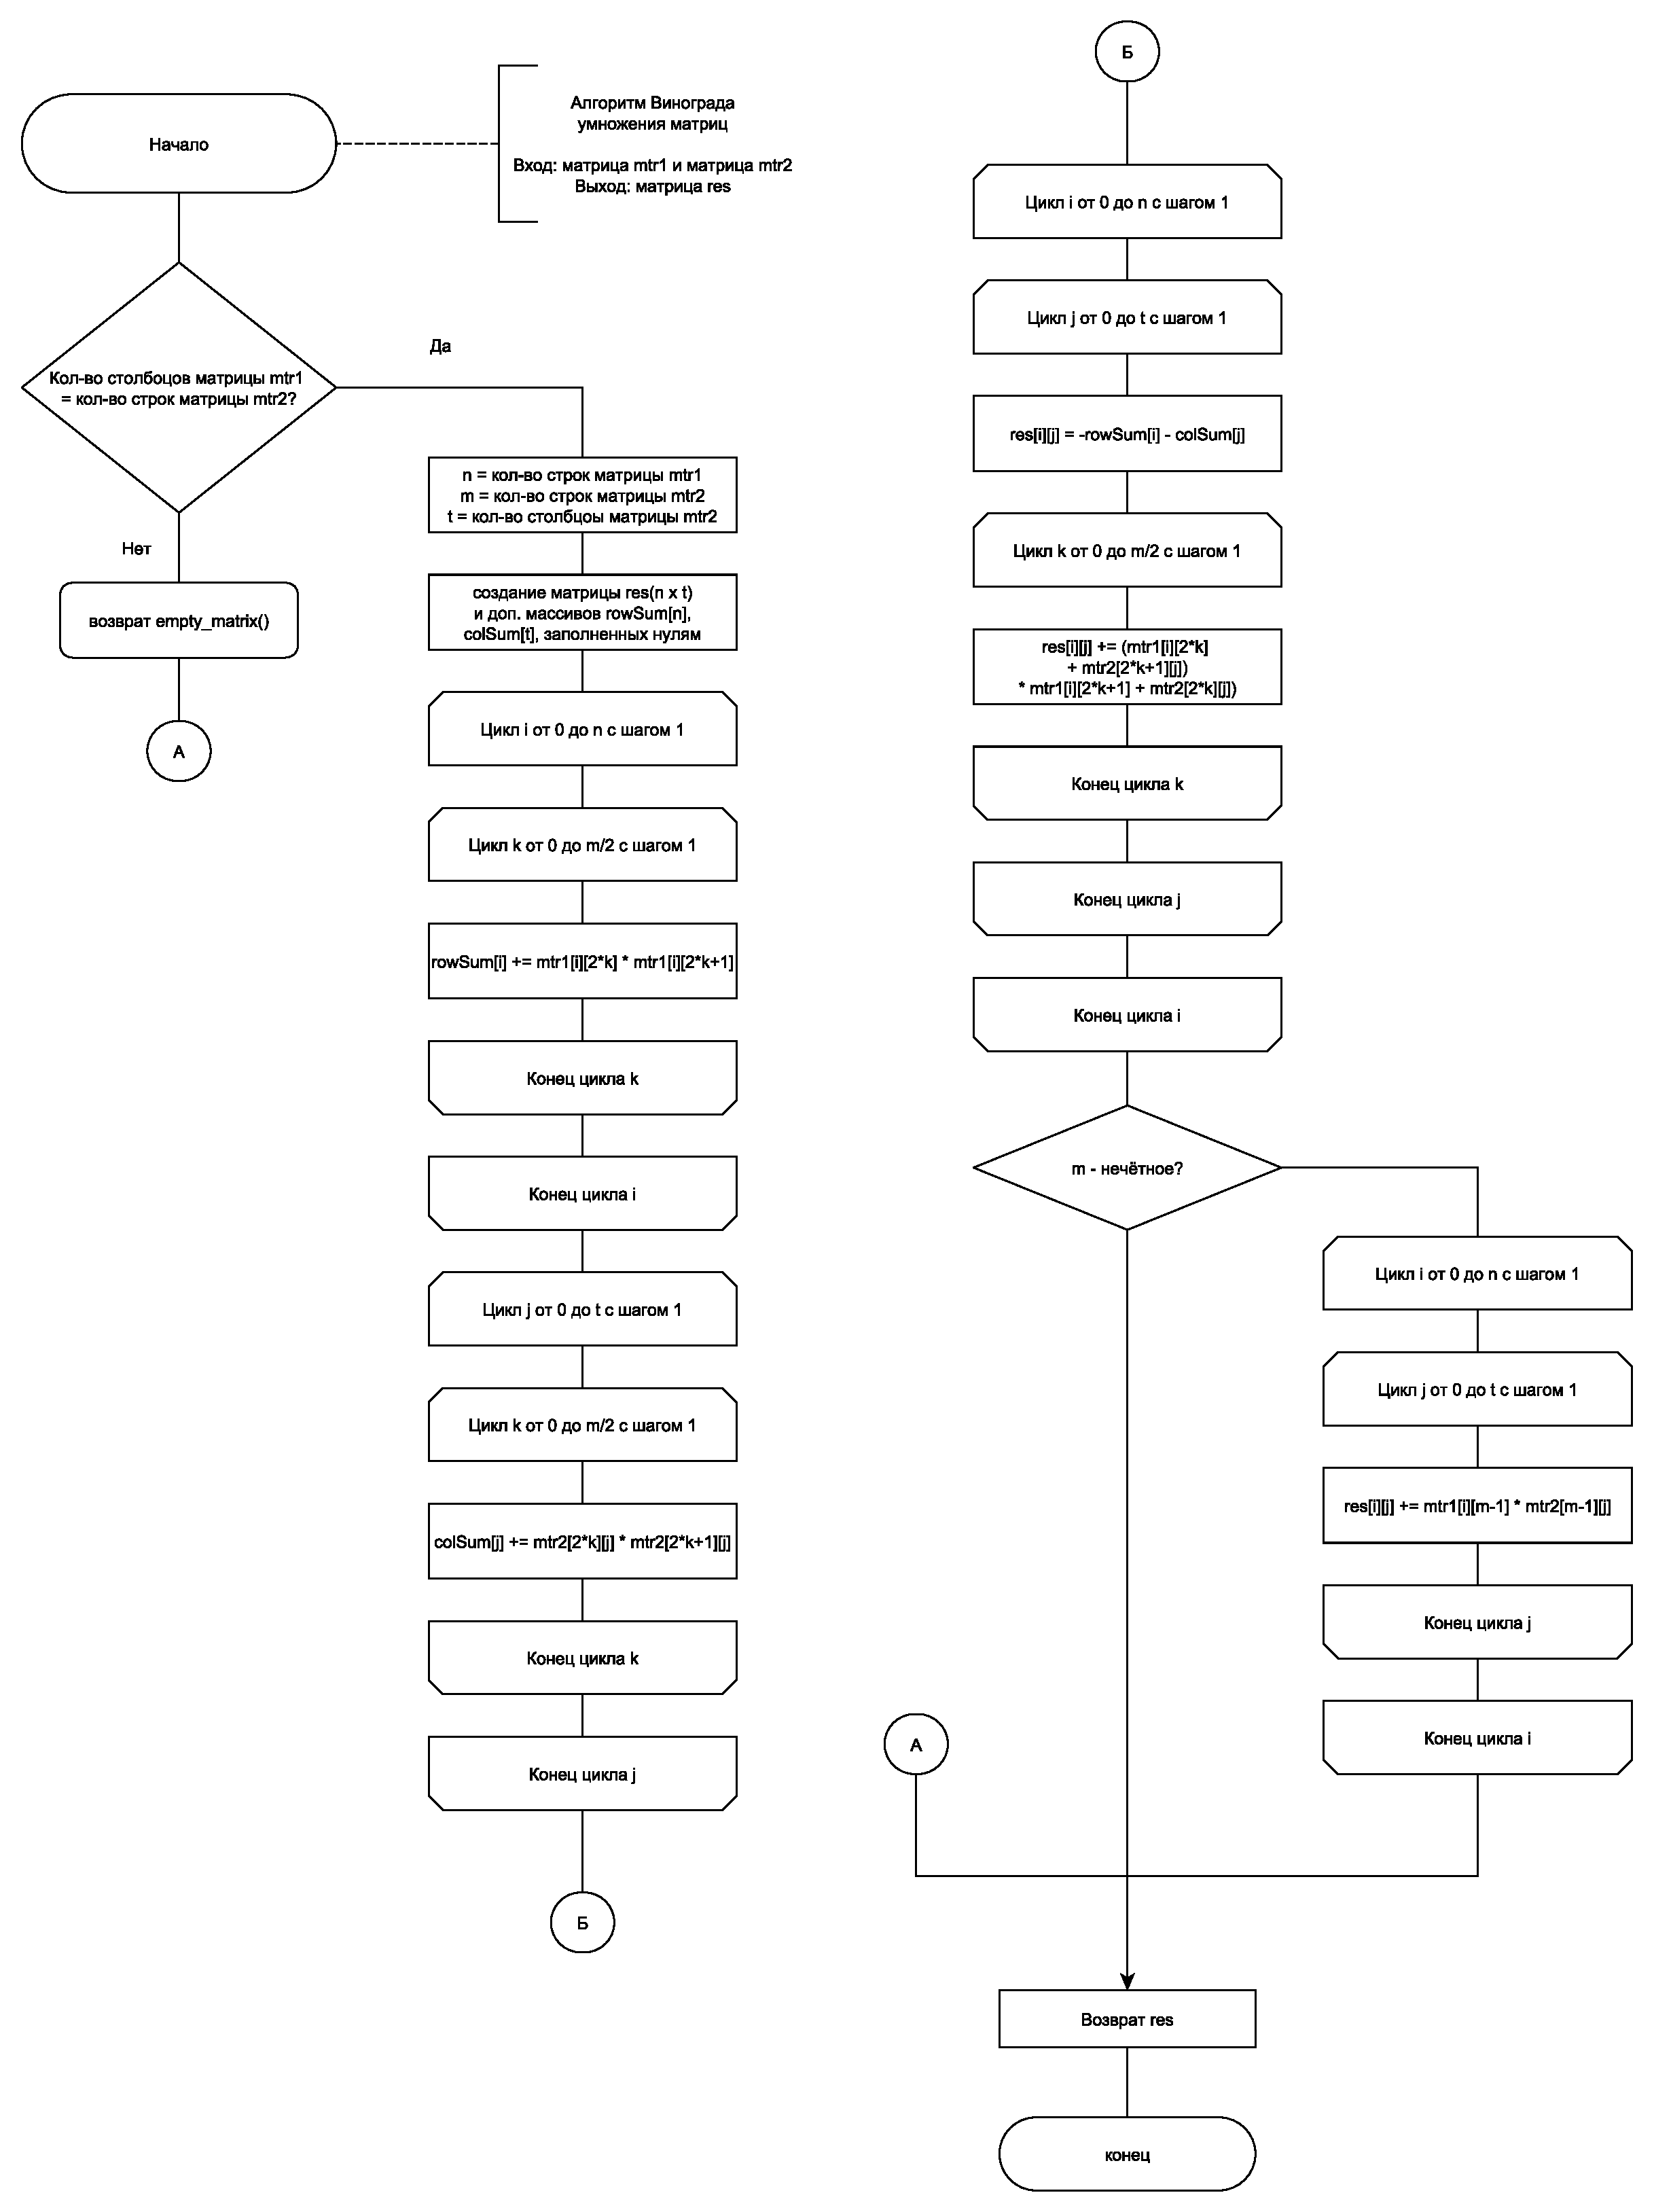
\includegraphics[width=1\linewidth]{images/shema_num2}
	\caption{Схема алгоритма Винограда умножения матриц}
	\label{fig:shemanum2}
\end{figure}

\begin{figure}[h]
	\centering
	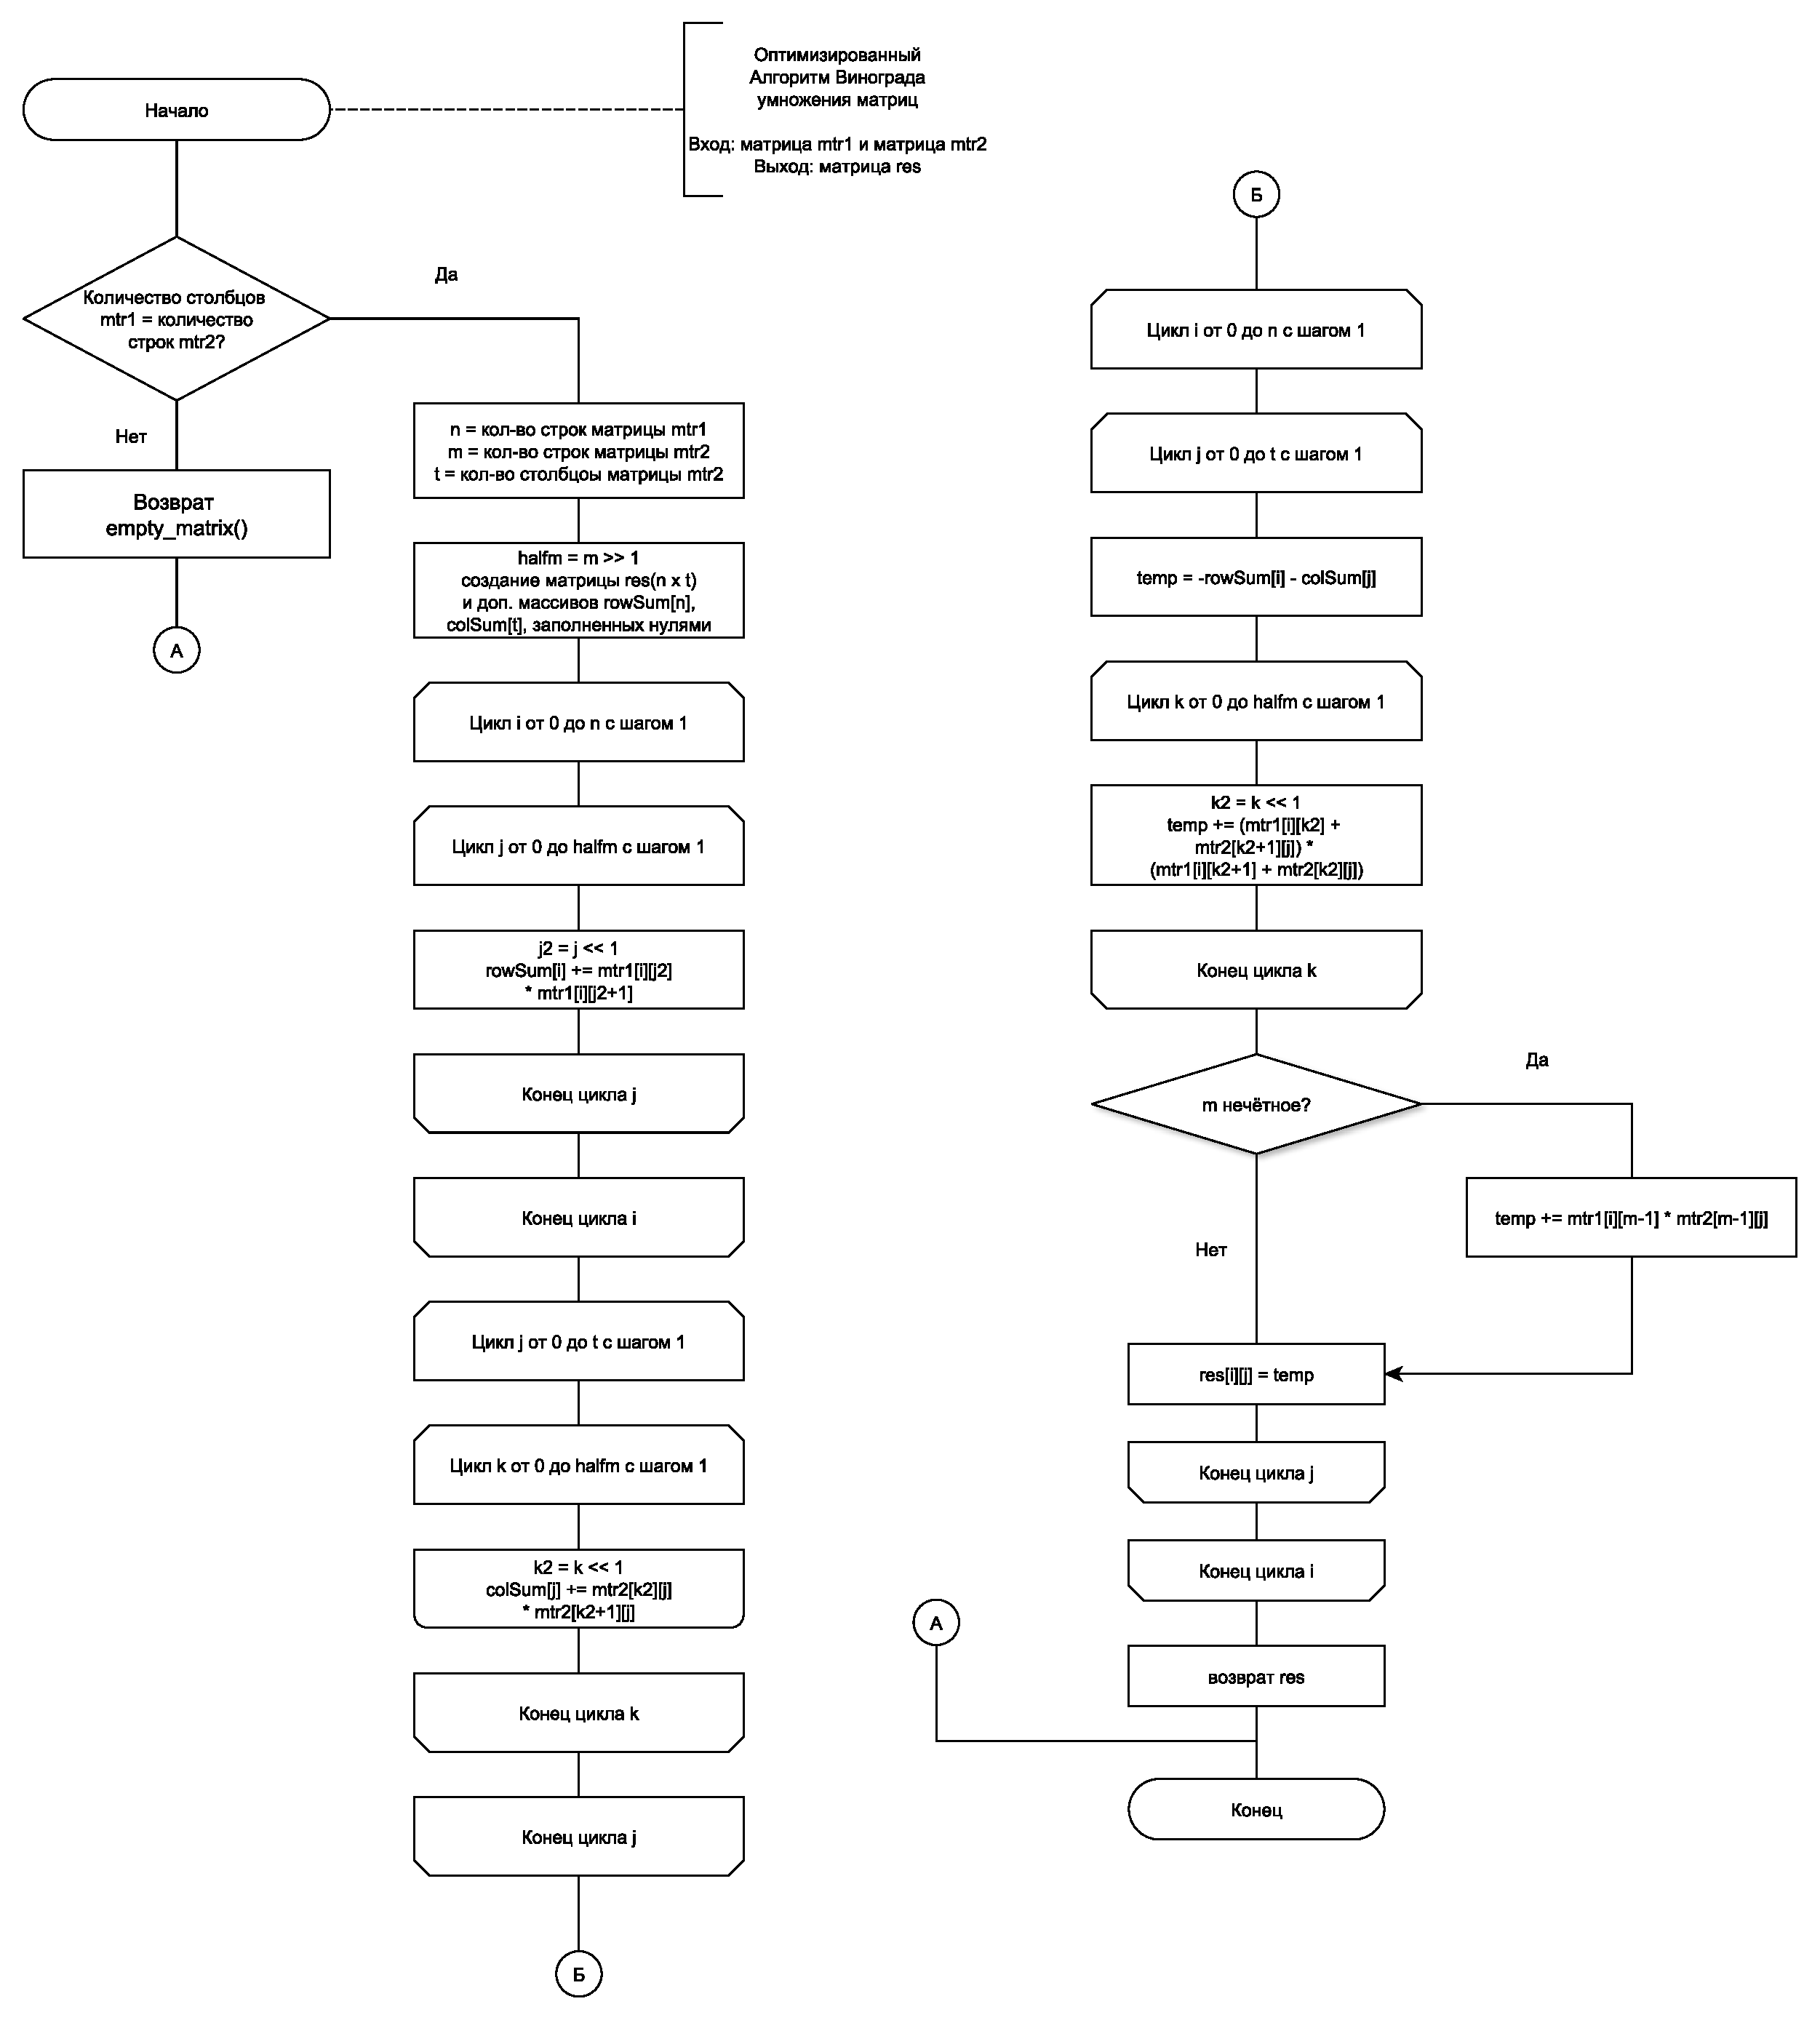
\includegraphics[width=1\linewidth]{images/shema_num3}
	\caption{Схема оптимизированного алгоритма Винограда умножения матриц}
	\label{fig:shemanum3}
\end{figure}

\clearpage

\section{Модель вычислений}

Для последующего вычисления трудоемкости необходимо ввести модель вычислений:

\begin{enumerate}
	
	\item операции из списка (\ref{for:operations}) имеют трудоёмкость 1;
	
	\begin{equation}
		\label{for:operations}
		+, -, *, /, \%, ==, !=, <, >, <=, >=, [], ++, {-}-
	\end{equation}
	
	\item трудоёмкость условного оператора \textbf{if} рассчитывается по формуле (\ref{for:if});
	
	\begin{equation}
		\label{for:if}
		f_{if} = f_{\text{условия}} +
		\begin{cases}
			\min(f_A, f_B), & \text{если условие выполняется}, \\
			\max(f_A, f_B), & \text{иначе}.
		\end{cases}
	\end{equation}
	
	\item трудоёмкость цикла рассчитывается как (\ref{for:for});
	
	\begin{equation}
		\label{for:for}
		f_{for} = f_{\text{инициализации}} + f_{\text{сравнения}} + N(f_{\text{тела}} + f_{\text{инкремента}} + f_{\text{сравнения}})
	\end{equation}
	
	\item трудоёмкость вызова функции/возврата результата равна 0;
	
\end{enumerate}

\section{Трудоёмкость алгоритмов}

В следующих частях будут расчитаны трудоемкости алгоритмов умножения матриц.
Также не будет учитываться инициализация матрицы результата, потому что данное действие есть во всех алгоритмах и при этом не является самым трудоёмким.

\subsection{Стандартный алгоритм умножения матриц}

Для расчёта трудоёмкости воспользуемся следующими обозначениями:

\begin{itemize}
	\item[---] n --- кол-во строк первой матрицы;
	\item[---] m --- кол-во столбцов первой матрицы и кол-во строк второй матрицы;
	\item[---] t --- кол-во столбцов второй матрицы;
\end{itemize}

Трудоёмкость стандартного алгоритма умножения матриц состоит из:

\begin{itemize}
	\item[---] внешнего цикла по $i \in [0..n)$, трудоёмкость которого: $f = 2 + n \cdot (2 + f_{\text{body}})$;
	\item[---] цикла по $j \in [0..t)$, трудоёмкость которого: $f = 2 + t \cdot (2 + f_{\text{body}})$;
	\item[---] цикла по $k \in [0..m)$, трудоёмкость которого: $f = 2 + 10 \cdot m$;
\end{itemize}

Учитывая, что трудоёмкость стандартного алгоритма равна трудоёмкости внешнего цикла:
\begin{equation}
	\label{for:classic}
	f_{\text{classic}} = 2 + n \cdot \bigl(4 + m \cdot (4 + 10t)\bigr) = 2 + 4n + 4nm + 10nmt 
\end{equation}

Для квадратных матриц (\( n = m = t \)) формула (\ref{for:classic}) принимает вид:

\begin{equation}
	\label{for:classic_square}
	f_{\text{classic}} = 2 + 4n + 4n^2 + 10n^3
\end{equation}

\subsection{Алгоритм Винограда}

Чтобы вычислить трудоёмкость алгоритма Винограда, нужно учесть следующее:
\begin{itemize}
	
	\item[---] трудоёмкости создания и инициализации вспомогательных массивов \texttt{rowSum} и \texttt{colSum}, равной (\ref{for:init});
	\begin{equation}
		\label{for:init}
		f_{\mathrm{init}} = n + t
	\end{equation}
	
	\item[---] трудоёмкости заполнения массива \texttt{rowSum}, равной (\ref{for:rowsum});
	\begin{equation}
		\label{for:rowsum}
		f_{\mathrm{rowSum}} = 2 + n \left( 2 + \frac{m}{2} \cdot 11 \right)
	\end{equation}
	
	\item[---] трудоёмкости заполнения массива \texttt{colSum}, равной (\ref{for:colsum});
	\begin{equation}
		\label{for:colsum}
		f_{\mathrm{colSum}} = 2 + t \left( 2 + \frac{m}{2} \cdot 11 \right)
	\end{equation}
	
	\item[---] трудоёмкости основного цикла вычисления результата для чётной части внутренней размерности, равной (\ref{for:cycle});
	\begin{equation}
		\label{for:cycle}
		f_{\mathrm{cycle}} = 2 + n \left( 4 + t \left( 11 + \frac{m}{2} \cdot 23 \right) \right)
	\end{equation}
	
	\item[---] трудоёмкости дополнительного цикла при нечётной внутренней размерности, равной (\ref{for:last});
	\begin{equation}
		\label{for:last}
		f_{\mathrm{last}} =
		\begin{cases}
			2, & \text{если } m \text{ чётно}, \\
			4 + n \left( 4 + 14t \right), & \text{если } m \text{ нечётно}.
		\end{cases}
	\end{equation}
\end{itemize}

Подставив формулы (\ref{for:init})–(\ref{for:last}), получаем итоговую трудоёмкость алгоритма Винограда в худшем случае (\( m \) нечётно):

\begin{equation}
	\label{for:vinograd_full}
	f_{\text{Винограда}} = 13 + 8n + 4t + \frac{11}{2}nm + \frac{11}{2}tm + 11nt + \frac{23}{2}nmt + 4 + 4n + 14nt
\end{equation}

Упростим выражение:

\begin{equation}
	\label{for:vinograd_simplified}
	f_{\text{Винограда}} = 17 + 12n + 4t + \frac{11}{2}nm + \frac{11}{2}tm + 25nt + \frac{23}{2}nmt
\end{equation}

Для квадратных матриц (\( n = m = t \)) формула (\ref{for:vinograd_simplified}) принимает вид:

\begin{equation}
	\label{for:vinograd_square}
	f_{\text{Винограда}} = 17 + 12n + 4n + \frac{11}{2}n^2 + \frac{11}{2}n^2 + 25n^2 + \frac{23}{2}n^3
\end{equation}

\begin{equation}
	\label{for:vinograd_final}
	f_{\text{Винограда}} = 17 + 16n + 36n^2 + \frac{23}{2}n^3
\end{equation}

\subsection{Оптимизированный алгоритм Винограда}

Оптимизация заключается в:

\begin{itemize}
	\item использовании побитового сдвига вместо умножения на 2;
	\item объединении цикла для нечётного размера матрицы с основным циклом — дополнительные вычисления при нечётном значении $m$ теперь выполняются внутри него;
	\item замене операций деления и взятия остатка на побитовые операции (\texttt{m >> 1} вместо \texttt{m / 2}, \texttt{m \& 1} вместо \texttt{m \% 2}); \newline
\end{itemize}

Тогда трудоёмкость оптимизированного алгоритма Винограда состоит из:

\begin{itemize}
	\item[---] трудоёмкости предварительного вычисления значения \texttt{halfm = m >> 1}, равной (\ref{for:opt_half});
	\begin{equation}
		\label{for:opt_half}
		f_{\mathrm{half}} = 1
	\end{equation}
	
	\item[---] трудоёмкости создания и инициализации массивов \texttt{rowSum}, \texttt{colSum} и результата \texttt{res}, равной (\ref{for:opt_init});
	\begin{equation}
		\label{for:opt_init}
		f_{\mathrm{init}} = 5 + 2n + 2t
	\end{equation}
	
	\item[---] трудоёмкости заполнения массива \texttt{rowSum}, равной (\ref{for:opt_rowsum});
	\begin{equation}
		\label{for:opt_rowsum}
		f_{\mathrm{rowSum}} = 2 + n \left( 2 + \frac{m}{2} \cdot 10 \right):
	\end{equation}
	
	\item[---] трудоёмкости заполнения массива \texttt{colSum}, равной (\ref{for:opt_colsum});
	\begin{equation}
		\label{for:opt_colsum}
		f_{\mathrm{colSum}} = 2 + t \left( 2 + \frac{m}{2} \cdot 10 \right)
	\end{equation}
	
	\item[---] трудоёмкости основного цикла вычисления результата, включающего обработку нечётного случая, равной (\ref{for:opt_cycle});
	\begin{equation}
		\label{for:opt_cycle}
		f_{\mathrm{cycle}} = 2 + n \left( 4 + t \left( 10 + \frac{m}{2} \cdot 22 + f_{\mathrm{odd}} \right) \right),
	\end{equation}
	где \( f_{\mathrm{odd}} \) — трудоёмкость дополнительных операций при нечётном \( m \), равная:
	\begin{equation}
		\label{for:opt_odd}
		f_{\mathrm{odd}} =
		\begin{cases}
			0, & \text{если } m \text{ чётно}, \\
			4, & \text{если } m \text{ нечётно}.
		\end{cases}
	\end{equation}
\end{itemize}

Подставив формулы (\ref{for:opt_half})–(\ref{for:opt_odd}), получаем итоговую трудоёмкость оптимизированного алгоритма Винограда в худшем случае (\( m \) нечётно):

\begin{equation}
	\label{for:opt_full}
	f_{\text{опт. Винограда}} = 12 + 8n + 4t + 5nm + 5tm + 14nt + \frac{23}{2}nmt
\end{equation}

Для квадратных матриц (\( n = m = t \)) формула (\ref{for:opt_full}) принимает вид:

\begin{equation}
	\label{for:opt_square}
	f_{\text{опт. Винограда}} = 9 + 11n + 19n^2 + \frac{9}{2}n^3
\end{equation}

\section*{Вывод}

В данном разделе были представлены схемы алгоритмов умножения матриц, а также были проведены расчёты трудоёмкости каждого из трём алгоритмов.

\clearpage